% Version 1: Bernd
% Version 2: Omar
% Version New: Bernd
\documentclass[usenatbib,usegraphicx,useAMS,onecolumn]{mn2e}
\usepackage[T1]{fontenc}
%\usepackage{txfonts}
\usepackage{multirow}
\usepackage[dvipsnames]{xcolor}
\usepackage{times}
\usepackage{amssymb}
\usepackage{listings}
\usepackage{enumitem}
\usepackage{tcolorbox}
\newcommand{\COzero}{${}^{12}\mathrm{CO}(1-0)$}
\newcommand{\COtwo}{${}^{12}\mathrm{CO}(2-1)$}
\newcommand{\Fe}{\textsc{feii}}
\newcommand{\Ox}{\textsc{[oiii]}}
\newcommand{\Ni}{\textsc{[nii]}}
\newcommand{\Su}{\textsc{[sii]}}
\newcommand{\Hb}{\mbox{H$\beta$}}
\newcommand{\Ha}{\mbox{H$\alpha$}}
\newcommand{\HII}{\textsc{hii}}
\newcommand{\QDeb}{\textsc{qdeblend${}^{\mathrm{3D}}$}}
\newcommand{\changed}[1]{\textbf{#1}}
%\newcommand{\changed}[1]{#1}
\newcommand{\pasp}{PASP}
\newcommand{\aj}{AJ}
\newcommand{\apj}{ApJ}
\newcommand{\apjs}{ApJS}
\newcommand{\aap}{A\&A}
\newcommand{\aaps}{A\&AS}
\newcommand{\araa}{ARA\&A}
\newcommand{\mnras}{MNRAS}
\newcommand{\apjl}{ApJL}
\lstset{basicstyle=\footnotesize\ttfamily, breaklines=true}
\newcommand{\codeline}[1]{\lstinline|#1|}
\newcommand{\paramdef}[1]{\textcolor{red}{\codeline{#1}}}
\newcommand{\tblcol}[1]{\textcolor{blue}{\codeline{#1}}}
\newcommand{\fname}[1]{\textcolor{magenta}{\codeline{#1}}}
\newcommand{\headerkw}[1]{\textcolor{ForestGreen}{\codeline{#1}}}
\newcommand{\headerval}[1]{\textcolor{YellowGreen}{\codeline{#1}}}
\newcommand{\PyPar}{\mbox{\textsc{PyParadise}}}
\newcommand{\myemail}{husemann@mpia.de}
%\bibpunct{(}{)}{;}{a}{}{,}


\definecolor{deepblue}{rgb}{0,0,0.5}
\definecolor{deepred}{rgb}{0.6,0,0}
\definecolor{deepgreen}{rgb}{0,0.5,0}
\setlength\parindent{0pt}

\begin{document}

\title{PyParadise User Manual}

\author[Husemann et al.]{B.~Husemann$^{1}$, O. S. Choudhury$^{2}$, C. J. Walcher$^{2}$\newauthor\\
$^1$European Southern Observatory, Karl-Schwarzschild-Str. 2, 85748 Garching b. M\"unchen, Germany\\
$^2$Leibniz-Institut f\"ur Astrophysik Potsdam (AIP), An der Sternwarte 16, 14482 Potsdam, Germany\\
}
\maketitle
\begin{abstract}

\end{abstract}
%\begin{keywords}
%\end{keywords}

\section{Installation}
\label{sec:installation}
\subsection{Software dependencies}
\PyPar\ depends on the following software:
\begin{itemize}
    \item python version 2.7 or 3.X
    \item numpy, version 1.12.1 or later
    \item scipy, version 0.19.0 or later
    \item astropy, version 2.X or later
\end{itemize}
For the MCMC algorithm two options are available of which only one needs to be installed:
\begin{itemize}
    \item pymc, version 2.3.6 or later
    \item emcee, version 2.2.1 or later
\end{itemize}

While different combination of package version may work as well, we suggest to create a dedicated python environment with miniconda (https://docs.conda.io/en/latest/miniconda.html). All packages can be easily install within the conda environment using the command 
\begin{lstlisting}[language=sh]
    conda install PACKAGE=VERSION
\end{lstlisting}
This allows the user to select the necessary specific versions described above to be installed under a common environment. This ensures stable operations of \PyPar. Running \PyPar\ with different version than the once listed above is at the users risk.


\subsection{Package Installation}
In order to install \PyPar, you can obtain the code from BitBucket, and install by running the following command from the main directory (ideally within the prepared conda environment)
\begin{lstlisting}[language=sh]
    python setup.py install
\end{lstlisting}
If the user does not want to create a dedicate environment with conda, you need to consider running the command with superuser-permissions or to change the command to either of the following commands
\begin{lstlisting}[language=sh]
    python setup.py install --user
    python setup.py install --home
\end{lstlisting}
while the preferred option is clearly the first, the second option requires a correct setup of the \codeline{PYTHONPATH} environment variable.

\subsection{Spectral stellar population templates library and example files}
\PyPar\ is shiped with several spectral stellar population template libraries and some example files with the purpose to get the user familiar with the necessary parameter files, input files and output files. \bigskip\\
\textbf{Important:} The installation procedure \textbf{will not} copy the template files nor the example files to a new location, but will stay in the \fname{templates} and \fname{examples} directory. The user is free to move thes files to any location. The location of the template files will be specified in the parameter files and is totally independent of the internal \PyPar\ installation directory.

\section{Quick start}\label{sec:quickstart}
Please read this section if you want to start working with \PyPar\ quickly. This section provides the minimum information to run \PyPar\ successfully on a certain data set. It is based on the example files provided with \PyPar\ and we recommend that new users first run \PyPar\ on the example files and have a careful look at them before applying \PyPar\ to their own data. More details on the algorithms and full explanations on all parameters and functionality is given in Sect.~\ref{}. For the most common mistakes we refer to the toubleshooting Sect.~\ref{sec:trouble} for further details.

\subsubsection{List of distributed files and their purpose}


\subsection{Running \PyPar}
\PyPar\ can be applied on single spectra, a collection of spectra (i.e. row-stacked spectra or RSS), and a 3-dimensional cube from integral field spectroscopy. The necessary data format for all three cases is explained in Sect.~\ref{sec:data}. Below we provide the sequence of commands to process the example RSS file \fname{NGC2691.COMB.RSS.fits}.\\
The \textbf{stellar continuum fit}
\begin{lstlisting}[language=sh]
    ParadiseApp.py NGC2691.COMB.RSS.fits NGC2691 6.0 --SSP_par parameters_stellar --parallel 1
\end{lstlisting}

\noindent The \textbf{emission line fit} in the residual spectra
\begin{lstlisting}[language=sh]
    ParadiseApp.py NGC2691.COMB.RSS.fits NGC2691 6.0 --line_par parameters_eline --parallel 1
\end{lstlisting}

\noindent The \textbf{bootstrap run to construct proper errors} for all parameters
\begin{lstlisting}[language=sh]
    ParadiseApp.py NGC2691.COMB.RSS.fits NGC2691 6.0 --SSP_par parameters_stellar --line_par parameters_eline --bootstraps 100 --parallel 4
\end{lstlisting}

\noindent In the command lines above \fname{NGC2691} is a output file prefix, \fname{6.0} is the spectral resolution of the input spectra in unit wavelength (FWHM), \fname{parameter_stellar} and \fname{parameters_eline} are setup parameter files. The number of CPU cores to be used is given by the \fname{--parallel}  and the size of bootstrap sample is given by the \fname{--bootstraps} command line parameters.

\subsection{Basic content of output files}
Once the user ran the commands as indicated in the above example several output file will occur for the three stages. 
\subsubsection{Stellar continuum fit result}
The best-fit stellar continua spectra and the residual spectra are stored as a FITS image in the files \fname{<PREFIX>.cont_model.fits} and \fname{<PREFIX>.cont_res.fits} with the same dimension as in the input data. An example for the resulting stellar continuum model for the test case \fname{NGC2691} is shown in Fig.~\ref{fig:NGC2691_example}. 

In addition, a FITS table \fname{<PREFIX>.stellar_table.fits} is stored which lists inferred measurements from the best-fit for each spectrum. It contains the stellar kinematic parameters including errors from the MCMC run and various stellar population parameters such as luminosity-weighted age (\fname{lum\_age\_total}) or luminosity-weighted iron abundance (\fname{lum\_[Fe/H]\_total}). We highly recommend to use the software \textsc{TOPCAT} (http://www.star.bris.ac.uk/$\sim$mbt/topcat/) to quickly visualize the output table content. 

\subsubsection{Emission line fit result}
The best-fit emission-line model and the residual spectra are stored as a FITS image in the files \fname{<PREFIX>.eline_model.fits} and \fname{<PREFIX>.eline_res.fits} with the same dimension as in the input data. An example of the resulting emission line model for the test case \fname{NGC2691} is shown in Fig.~\ref{fig:NGC2691_example}. 

In addition, a FITS table \fname{<PREFIX>.eline_table.fits} is stored which lists inferred measurements from the best-fit for each spectrum. For all fitted lines it lists the  line flux \fname{<LINE>\_flux}, line velocity \fname{<LINE>\_vel} in km/s, and intrinsic line width \fname{<LINE>\_fwhm} in km/s. 

\subsubsection{Bootstrap error estimation result}
The bootstraps run repeats the measurements for each spectrum $N$ times as specified in the \fname{--bootstraps <N>} parameter. In each repetition the input spectrum is randomly modulated within the associated error budget and only a random subsect from the template spectral library is use to model the spectrum.

Errors on each parameter are derived by taking a standard deviation of the repeated measurements and assumming a normal distribution. The tables \fname{<PREFIX>.stellar_table.fits} and \fname{<PREFIX>.eline_table.fits} are expanded with additional error columns for each parameter and columns names \fname{<COLUMN>_err}. 

\begin{figure}
 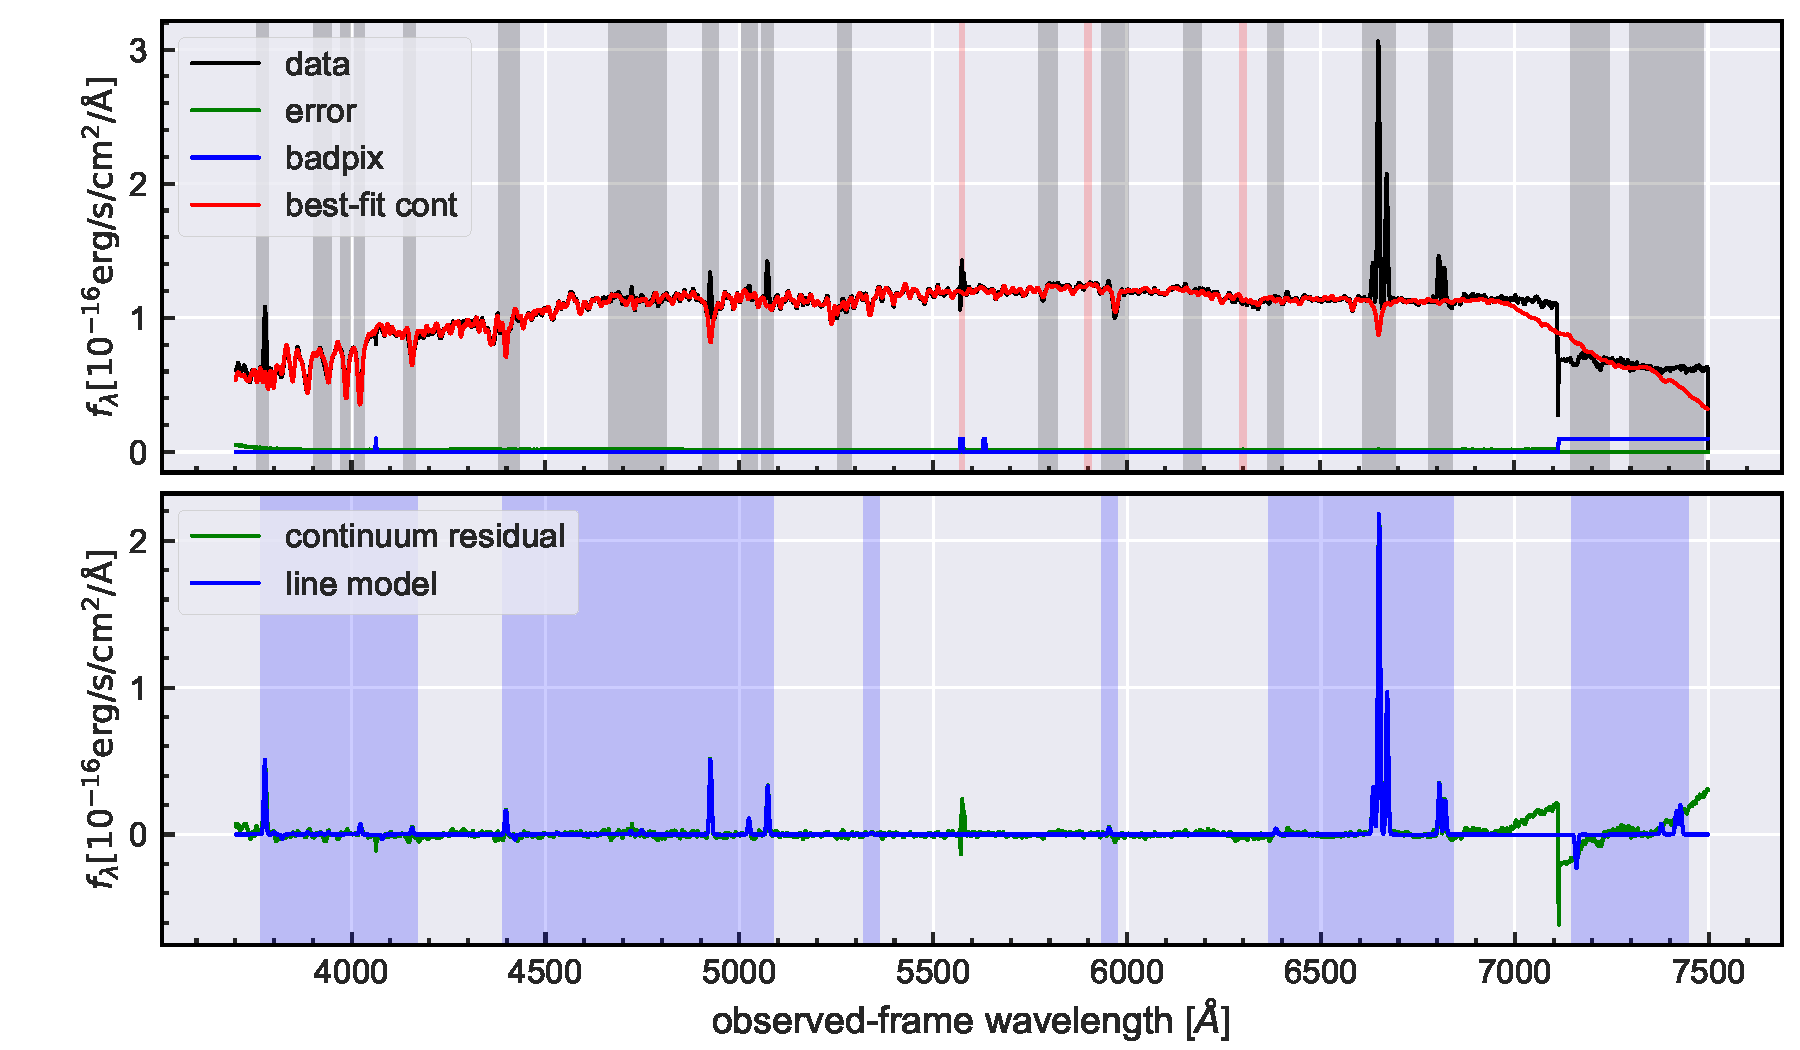
\includegraphics[width=\textwidth]{figs/example_spec/NGC2619_COMB_RSS_0.pdf}
  \caption{\PyPar\ results for the first spectrum in the provided RSS file \fname{NGC2619.COMB.RSS.fits}. The upper panel shows the best fit stellar continuum with respect to the observed data and associated errors an bad pixel flag (==0 if good pixel). The grey and red area highlight wavelength regions masked out in the rest frame (for emission lines) and observed frame (for sky lines), respectively. The lower panel shows the best-fit emission line model with single Gaussians coupled in redshift and line dispersion. The blue area highlights the wavelength regions which are taken into accout to compute the $\chi^2$ for the fitting of emission lines. Failure of providing a mask that does not cover all emission line components will results in wrong results.}\label{fig:NGC2691_example}
\end{figure}


\subsection{Quick visualization of results}

\subsection{A quick look at the necessary parameter files}
To successfully run \PyPar\ a correct setup of the necessary parameters are crucial. Most of the parameters may only be changed by expert users and can be left safely unchanged for most circumstances. We refer to Sect.~\ref{} to gain deep insight into the underlying algorithms and purpose of all parameters that can be set to optimize \PyPar. Below we briefly explain the necessary files to run \PyPar\ and should be available in the example directory:
\begin{itemize}
 \item \fname{NGC2691.COMB.RSS.fits} $\rightarrow$ Input spectral data to fit
 \item \fname{parameters\_stellar} $\rightarrow$ Parameter file for stellar continuum fit
 \item \fname{excl.cont} $\rightarrow$ Wavelength mask for continuum normalization
 \item \fname{excl.fit} $\rightarrow$ Wavelength mask for continuum fitting
 \item \fname{parameters\_eline} $\rightarrow$ Parameter file for emission line fit
 \item \fname{par.lines} $\rightarrow$ Definition of line component model
 \item \fname{lines.fit} $\rightarrow$ Wavelength region considered for emission-line fit
\end{itemize}
Please check that all those files are available in the example directory of the downloaded package. 


\subsubsection{Example stellar continuum parameter file}
The parameter file for the continuum fit is an ASCII file which sets several important parameters. Each line defines a certain parameter with a parameter name,  a parameter value, and optionally followed by a comment separated with a '!' sign from the parameter. For the stellar contiuum fit an example parameter file \fname{parameters\_stellar} is available in the example directory. The most important parameters to be updated by the users are the following:\bigskip\\
\textcolor{red}{\codeline{tmpldir         ../Paradise/templates}}\\
\textcolor{red}{\codeline{tmplfile        CB09_templates.fits}}\\   
\textcolor{red}{\codeline{vel_guess       4040.0}}\\ 
\textcolor{red}{\codeline{vel_min         3900.0}}\\
\textcolor{red}{\codeline{vel_max         4200.0}}\\ 
\textcolor{red}{\codeline{start_wave      3701.0}}\\  
\textcolor{red}{\codeline{end_wave        7499.0}}\bigskip\\  
These parameters usually need to be updated for every data set by the user. The absolute or relative path to the templates directory containing the stellar continuum template library \fname{tmpldir} need to be set properly. Ideally a common absolute path is set and re-used for a given computer. The spectral library template file \fname{tmplfile} need to be specified \textbf{and must exist in the specified template directory}. It is crucial to set a good guess \fname{vel\_guess} for the mean systemic redshift of the input spectra expressed in km/s as $cz$. The MCMC algorithm is only exploring the stellar kinematics within certain bondaries, so the minimum \fname{vel\_min} and maximum \fname{vel\_max} velocities around the systemic one needs to be chosen. Depending on the wavelength range covered and whether only a partial wavelength range should be modelled, the start \fname{start\_wave} and end \fname{end\_wave} wavelength. All other parameters can be left unchanged except the user is familiar with the details of parameters, explained in the Sect.~\ref{}, and known the consequences.


\subsubsection{Example emission line parameter file}
\PyPar\ can also fit Gaussian emission line profiles to the residual spectra after the best-fit continuum model is subtracted. Another parameter file is needed for this second processing step which has a similar syntax as the parameter file for the continuum fit. An exmple parameter file \fname{parameters_eline} is available in the example directory. From the file the most curcial lines to be updated by the users are:\bigskip\\
\textcolor{red}{\codeline{eCompFile  par_lines}}\\
\textcolor{red}{\codeline{vel\_guess   4040.0}}\\
\textcolor{red}{\codeline{eguess\_window 20}}\bigskip\\
Those parameters usually need to be updated for every data set by the user. A dedicated file is needed to describe the emission line model to be fitted. The absolute path/file name of this emission line components file is registered in the \fname{eCompFile} parameter. Similar to the stellar continuum model, the systemic redshift of the emission lines need to be set as an initial guess \fname{vel\_guess} expressed as $cz$ in km/s. In most case the same initially velocity guess as for the stellar continuum model can be used. The non-linear emission line fitting needs good starting values to converge. Those starting values for each Gaussian emission line component will be empirically determined from the spectra in pixel window around the redshifted central pixel of each emission line in the spectrum. This windows may be adjusted depending on the expected width of lines given based on spectral resolution and spectral sampling. 

\subsubsection{Emission line model file}
The associated model component file is a ASCII file that defines a list of different line components to be modelled. There is no limit on the number of components. Each component consistents of a block of several parameters depending on the specific component as described below. An example file \fname{par.lines} is available in the example directory.\bigskip\\
Each component block starts with a line that defines the component profile (i.e. Gaussian) and a unique component name (i.e. an identifier for the emission line). All parameters of the Gaussian such as flux, redshift (as velocity cz) and velocity dispersion in km/s, can also be tied to other lines based on the unique identifier. Also a factor to apply a fixed flux ratio is possible as indicated in case of the OIII doublet. \bigskip\\
The example file \fname{par.lines} lists a large number of potential emission lines of which a sub-sample of optical lines can be easily drawn for any specific case. For more complex situation and a full description of all features please read Sect.~\ref{} for more details on the line modelling.

\subsubsection{Wavelength selection files}
Certain wavelength windows need to be masked or selected at various instances during the fitting. Such spectral windows can be defined in an ASCII file either as spectral windows in the rest-frame (e.g. for emission lines) or observed-frame (e.g. for sky line residuals or detector artefacts). Examples of such spectral window files (\fname{excl.cont}, \fname{excl.fit}, \fname{lines.fit}) are available in the example directory.\bigskip\\

\PyPar\ requires three wavelength selection files for different purposes: 1) exclusion of emission lines, sky line residuals and detector artefacts during the continuum normalization $\rightarrow$ \fname{excl_cont} in \fname{parameter_stellar}, 2) exclusion of non-continuum emission for the actual stellar continuum fit $\rightarrow$ \fname{excl_fit} for \fname{parameter_stellar}, and 3) wavelength windows covering ALL emission lines to be fit $\rightarrow$ \fname{lines.fit} for \fname{parameter_eline}.  For most practical purposes \fname{excl_cont} and \fname{excl_fit} use the same spectral windows and can point to the same file for simplicity.\bigskip\\
\textbf{Important:} Failure in providing correct and complete wavelength selection files will usually lead to incorrect fitting of the spectra. This will be recognized as certain artefacts in the results. Some examples to identify common problems in the masking will be described in Sect.~\ref{}. 



\subsection{Available stellar template libraries}

\begin{tabular}{|l|c|c|c|c|c|c|}
 File name                     & spectra & coverage           & sampling & resolution & type & Reference\\\hline
 CB09\_templates.fits          &   85    &  3500\AA--9500\AA  & 0.9\AA   &  2.5\AA    & SSP  &          \\
 MIUSCAT\_BaSTI\_K\_baseFe.fits&   636   &  3465\AA--9470\AA  & 0.9\AA   &  2.5\AA    & SSP  &          \\
 RG04\_templates.fits          &    39   &  3001\AA--6998\AA  & 0.3\AA   &  0.6\AA    & SSP  &          \\
 INDO\_US\_random\_100.fits    &   100   &  3500\AA--9400\AA  & 0.4\AA   &  1.0\AA    & stars&    
\end{tabular}



%Copy the example template files from the test directory and adjust the path to the template directory accordingly.
%Update the \paramdef{vel_guess} parameter to a velocity close to the final velocity.
%Adjust the minimum and maximum values for the allowed ranges for the velocity $v$ and velocity dispersion $\sigma$.
%Have a look if the \paramdef{start_wave} and \paramdef{end_wave} contains the wavelength range where you want to perform the fitting.
%Similarly, make sure that \paramdef{min_x}, \paramdef{max_x} and \paramdef{min_y}, \paramdef{max_y} cut up your cube/rss file correctly.
%You can now run the stellar population fitting by running
%\begin{lstlisting}[language=sh]
%    ParadiseApp.py <input_file> <prefix> <spec_res> --SSP_par <ssp_par.txt>
%\end{lstlisting}
%which will produce the following three output files \fname{<prefix>.cont_model.fits}, \fname{<prefix>.cont_res.fits} and \fname{<prefix>.stellar_table.fits}.

\section{Stellar population modelling}\label{sec:ssp_model}
\subsection{\PyPar\ philosophie of fitting stellar continuum spectra}\label{subsec:ssp_algo}
The fitting of galaxy continuum spectra is a complex process and usually needs optimization of a highly multi-dimensional parameter space. All galaxy spectra can be described by the super-position of stellar template spectra which are convolved with the kinematics of the stars as described by a radial velocity (including cosmological redshift) and a velocity dispersion. Optimizing the mix of template spectra and the kinematics together is a non-linear optimization process.

\PyPar\ is breaking up the non-linear kinematic optimization and the linear super-position of template spectra into 2 indpendent steps using an iterative procedure. This has the advantage that only the few non-linear parameters are fitted with non-linear optimization methods, while the super-position of template spectra are preformed with very fast linear optimization methods. 

Since real spectra are never perfect and dust extinction may significantly affect the shape of the spectra and would not provide a good match to the any super-position of the template spectra. This issue is often solved by adding additional functions to the optimization, such as polynomials. However, even polynominals may not capture all the arteficial variation in the spectra correctly. Instead, \PyPar\ is normalizing the global continuum shape of the input spectra and template spectra in a non-parametric way before the algorithms is actually trying to match them.

\begin{tcolorbox}
\textbf{Important:} Due to the continuum normalization, \PyPar\ finds the best template super-position by reducing only the residuals of absorption line features and basically ignores the different continuum slopes of young and old stellar populations. Also the dust extinction cannot be determined during the fitting this way. Obviously this has clear advantages or disadvantages depending on the type of input spectra and the scientific objectives of the user. 
\end{tcolorbox}

\subsection{Template broadening to match instrumental spectral resolution}
The template library of continuum spectra has an intrinsic spectral resolution and spectral sampling, which is usually inhereted from the spectrograph the data are taken with. Before fitting the template spectra to the input data \PyPar\ therefore needs to match the spectral resolution by properly degrading the resolution of the template spectra, which is the first step in the process. Given that the input spectra are usually galaxy spectra with a significant redshift $z$, the redshifting of the templates need to be taken into account when computing the difference in spectral resolution of the templates ($\sigma_\mathrm{temp}$ in unit wavelength) and input data ($\sigma_\mathrm{data}(\lambda)$ in unit wavelength). The dispersion ($\sigma_\mathrm{smooth}$) of the Gaussian convolution kernel applied by \PyPar\ to the spectral template library is therefore given by
\begin{equation}
 \sigma_\mathrm{smooth}(\lambda) = \sqrt{\sigma_\mathrm{data}(\lambda)^2-\left(\left(1+\frac{v_\mathrm{guess}}{c}\right)\times \sigma_\mathrm{temp}\right)^2}
\end{equation}
Here, $v_\mathrm{guess}$ will be initially computed by \PyPar\ from the \fname{vel_guess} parameter in the \fname{parameter_stellar} stellar configuration file. 
While the templates spectra are usually generated such that the spectral resolution is constant with wavelength this may not be true for the input data. \PyPar\ is able to work with both cases and can adaptively adjust the width of the convolution kernel as a function of wavelength when smoothing the template library. When running \fname{PyParadiseApp.py} the user needs to provide a value for the spectral resolution of the data which can either be a single float number for the spectral resolution expressed in terms of Full Width at Half Maximum (FWHM) which is $\mathrm{FWHM}_\mathrm{data}=2.354\times\sigma_\mathrm{data}$, or the path to an ASCII file which describes the wavelength-dependent spectral resolution. The format of the file is rather simple with just two columns for the wavelength and the spectral resolution (FWHM). When applying the wavelengt-dependent spectral resolution, \PyPar\ is linearly interpolating the provide wavelength grid to the redshifted wavelength grid of the template spectra. The wavelength coverage in the file therefore needs to cover the entire wavelength range of the input spectra. An exmaple file for MUSE based on the measured wavelength-dependent spectral resolution \citep{} is available in the example directory with the name \fname{MUSE_spec_res.txt}.

\begin{tcolorbox}
 \textbf{Important}: When the spectral resolution of the redshifted template spectra become worse than the input data, a correct machting of the spectra becomes impossible. This would lead to an incorrect determinations of the stellar kinematics and possible wrong mix of template spectra. \PyPar\ will refuse to fit but provides the minimum spectral resolution of the redshfit template spectra according to \fname{vel_guess}. There are 2 options to solve that issue:
 \begin{itemize}
  \item select a template library of spectra with higher spectral resolution
  \item artifically set the input data spectral resolution to the redshifted spectral resolution of the templates
 \end{itemize}
\end{tcolorbox}

\subsection{Continuum normalization of input data and template spectra}
The next crucial step in the pre-fitting stage is the continuum normalization of the input data and the template spectra. This dependes crucially on masking all features that do not belong to the continuum such as emission lines, strong sky line residuals, detector artefact and bad pixels.  While bad pixels should already be provided with the input data (see Sect.~\ref{} for details of the input data format), wavelength regions covering emission lines and sky line residuals need to be defined by the user in the \fname{excl.cont} file as described in Sect.~\ref{} and available in the exmple directory. Here, wavelength windows can be defined in rest-frame and observed-frame seperately to aid the definition of masked wavelength regions.

The masked wavelength regions are then linearly interpolated to approximate a continuum singal in those regions. A running mean is then applied to the pure input spectra to create highly smooth version of the continuum shape. The with of the running mean average box size is set by the user in the \fname{nwidth_norm} parameter in the \fname{parameter_stellar} parameter file. The input spectra are then devided by their respective smoothed continuum spectra to achieve a normalization of the continuum close to 1 across the entire wavelength range. An example of the normalization process is shown in Fig.~\ref{}. The template spectra are similarly normalized after redshifting to \fname{vel_guess} and matching to the spectral resolution. Here, the box size of the running mean is automatically adjusted to match the same size in wavelength space based on the respective wavelength sampling of the input data and the template spectra. 

While the subsequent fitting is done with the continuum normalized spectra, the normalization information is stored throughout the process so that the results can be de-normalized at the end of the process to go back to normal space. 

\begin{tcolorbox}
 \textbf{Important:} The process crucially depends on propoer wavelength masks provided by the user. If artefact and emission lines are not properly masked in the input spectra, \PyPar\ will not be able to determine a good fit. It is therefore strongly encouraged, to review the definiation of the wavelength window by performing a test fit on a few characteristic spectra and use the visualization tools to check whether the provided wavelength masks are appropriate. General rule is that the wavelength regions should be broad enough to cover all non-continuum feature but small enough that enoug continuum signal remains to do a good continuum normalization. If the input spectra are nearly entirely dominated by non-continuum signal, \PyPar\ would not be the ideal software, but this is rarely the case.
\end{tcolorbox}




\subsection{Determination of stellar kinematics}\label{subsec:ssp_kin}
A Markov Chain Monte Carlo (MCMC) lies on the basis of the determination of the kinematics.
The constraints are the provided limits on the values that $v$ and $\sigma$ can take.
A random value for $v$ and $\sigma$ are taken between these limits, followed by a random walk consisting of $n$ steps.
At each step of the random walk, the code evaluates whether the new kinematical values improves or worsens the fit.
If the fit improves, the new values are accepted.

Stationarity is the state when the mean and variance for $v$ and $\sigma$ do not change when proceeding further in the walk.
The first set of steps inside a walk still depend strongly on the initial value and the MCMC is therefore not stationary for those steps.
These values need to be discarded, a process referred to as \textit{burn-in}.

Even with a proper burn-in, there can be some auto-correlation as the $v_i$ and $\sigma_i$ are based on the $v_{i-1}$ and $\sigma_{i-1}$.
When the auto-correlation is weak-to-moderate, the results from a small walk might be affected by auto-correlation.
For moderate-to-strong auto-correlation, the results from a longer walk might still be influenced by auto-correlation.
To counteract the auto-correlation, the chain can be \textit{thinned} by a factor $k$ by only taking every $k^{\rm th}$ sample of the chain.
This then produces a correction value to $v$ and $\sigma$, which are the values for the derived kinematics at this step of the random walk.

From the sample, $(n - m) / k$ points will be used to derive the mean and the errors of the $v$ and the $\sigma$.

\subsection{Super-position of template spectra}\label{subsec:ssp_ssp}
Before the stellar populations are fitted, there are a few preparatory steps.
Due to issues that often arise with in the data reduction and analysis of spectra, the continuum level is uncertain.
To address this problem, \textsc{PyParadise} normalises the input spectra and the template library before fitting.
To normalise the spectra a running mean is applied, with the width specified in the parameters-file.
Another option is to use a $n^{\rm th}$-order polynomial (not implemented yet), which is especially useful for data which has not been flux-calibrated yet.

The stellar population are fitted by applying a non-negative least squares (NNLS) algorithm when comparing a spectrum to the template library of model spectra.
It is non-negative as so far only light-emitting stellar population have been observed.
The template library does not consist of a set of spectra which are independent from each other, and the problem is referred mathematically as an ill-posed problem.
The NNLS therefore does not provide a unique solution and the recovery of the star-formation history using an NNLS algorithm usually only provides at most dozen non-zero weights, e.g. it tells that at most a dozen SSPs construct the full star-formation history of a galaxy.

We therefore provided a bootstrapping procedure, which re-fits the spectra a number of times with a subset of models.
If a contributing SSP in the fiducial fit is real and is removed during the bootstrapping procedure, it should be recovered by the similar SSPs during the bootstrapping.
See the paper for more details on recovery of stellar parameters from simulated galaxy spectra and a validation of bootstrapping to recover trustworthy star-formation histories.


\subsection{Best-fit sellar population parameters}

\subsection{Template handling}
\label{subsec:ssp_template}
\subsection{Masking}
\label{subsec:ssp_mask}
There are two different masking processes.
As the spectra are first normalized before the stellar populations are fitted, one needs to mask out regions which can impact the normalisation, hereafter referred as continuum masking.
What one wants to include for continuum masking are strong artefacts/residuals, strong emission lines and strong absorption lines.
The second masking involves features in the spectra which are not due to stellar populations features: this would be the emission lines and any artificial structure in the spectra.
The emission lines and artefacts are therefore masked twice, while the strong absorption lines are only masked out for the continuum determination.

\subsection{Parameters file}
\label{subsec:ssp_param}
\begin{itemize}
    \item \paramdef{tmpldir} (\texttt{string}) is the path to the directory in which the template file is located.
        This might be an absolute path or a relative path.
    \item \paramdef{tmplfile} (\texttt{string}) file contains all the template spectra, and should be formatted in the FITS format.
        There are two HDUs in the template file: the first one contains the spectra and the second one the stellar population parameters.
        The spectra in the first HDU unit are saved in RSS format, with $m$ wavelenegth elements along the first axis and the $n$ spectra along the second axis.
        The first wavelength element is given by the header keyword \textsc{CRVAL1}, the step in wavelength space by the header keyword \textsc{CDELT1}.
        
        In order to determine what the SSP parameters of each spectrum in the template file are, this information is located in the second HDU in table format.
        The $j^{\rm th}$ entry in the table has the SSP pararmeters corresponding to the $j^{\rm th}$ spectrum.
        This table should at least have the following columns:
        \begin{itemize}
            \item \tblcol{Luminosity}, which is the current luminosity of the SSP.
            \item \tblcol{Mass}, which is the current mass of the SSP, usually normalized such that the initial mass of the SSP is $1~M_{\odot}$.
            \item \tblcol{Age}, which is the age of the SSP.
            \item \tblcol{[Fe/H]}, which is the iron abundance of the SSP.
            \item \tblcol{[A/Fe]}, which is the [$\alpha$/Fe] abundance ratio of the SSP.
            \item \tblcol{mass-to-light}, which is used in the conversion of luminosity-weighted stellar population properties to mass-weighted stellar population properties.
        \end{itemize}
    \item \paramdef{tmplinitspec} (\texttt{int}) The initial spectrum to start the fitting with.
        A good guess can lead to a faster convergence, and a lower \paramdef{iterations} value might therefore be sufficient.
    \item \paramdef{vel_guess} (\texttt{float}). \paramdef{vel_guess} is the best guess for the systemic velocity corresponding to $cz$ for the object. 
    \item \paramdef{vel_min}, \paramdef{vel_max}, \paramdef{disp_min}, \paramdef{disp_max} (\texttt{float}).
        The parameters \paramdef{vel_min} and \paramdef{vel_max} are the absolute upper and lower velocity boundaries expressed as $cz_\mathrm{min}$ and $cz_\mathrm{max}$ in km/s, respectively, which define the search range for systemtic velocity during MCMC iteration. The \paramdef{disp_min} and \paramdef{disp_max} values similarly define the absolute boundaries for $\sigma$ in km/s.
    \item \paramdef{kin_fix} (0 or 1)
        If the \paramdef{kin_fix} parameter is set to 1, the kinematics will not be fitted, but will instead be read from \fname{<prefix>.kin_table.fits}.
        This table is located as the second HDU unit, and should have the values for the kinematics of each spectrum in the columns named \tblcol{vel_fit} and \tblcol{disp_fit}.
    \item \paramdef{excl_fit} (\texttt{string})
        Path to the file which contains the wavelength windows to exclude during the stellar absorption line fitting.
        This may be an absolute path or a relative path.
    \item \paramdef{excl_cont} (\texttt{string})
        Path to the file which contains the wavelength windows to exclude during the determination of the stellar continuum.
        This may be an absolute path or a relative path.
    \item \paramdef{nwidth_norm} (\texttt{int})
        The width of the running mean in pixel space in which the continuum will be determined.
    \item \paramdef{start_wave}, \paramdef{end_wave} (\texttt{float})
        These wavelength limits describe between where the spectra are fitted.
        One can also use the exclusion files for reducing the wavelength space, but the advantage of \paramdef{start_wave} and \paramdef{end_wave} is that the template spectra are truncated between these wavelength limits.
        As it reduces the wavelength range where the spectra are normalizes, it accelerates the computation and the reduced wavelength range reduces the memory footprint of the code.
    \item \paramdef{min_x}, \paramdef{max_x}, \paramdef{min_y}, \paramdef{max_y}
        If the input spectrum is in cube-format, these parameters extract a smaller cube and fit only those spectra.
        So if a cube has the shape (30, 40, 200), there are 30 spectra along the x direction times 40 spectra along the y direction, and each spectrum contains 2000 wavelength elements.
        If \paramdef{min_x} and \paramdef{max_x} are set to 10 and 15, respectively, and \paramdef{min_y} and \paramdef{max_y} are set to 3 and 5 respectively, only the spectra along (10:15, 3:5) are fitted.
    \item \paramdef{iterations} (\texttt{int})
        The fitting of the best (combination of) SSP(s) amd the kinematics are two different computational steps.
        At the first iteration, the \paramdef{tmplinitspec} is used to fit the kinematics.
        The kinematics obtained from this is then applied to the template library and the best-ftting (combination of) SSP(s) are obtained, which gives the SSP parameters and the best-fitted spectrum.
    \item \paramdef{samples} (\texttt{int})
        The total number of random walks performed inside an MCMC chain. 
        The longer the chain, the more reliable becomes the determination of $v$ and $\sigma$. 
    \item \paramdef{burn} (\texttt{int})
        An MCMC chain starts from a random value between \paramdef{vel_min} and \paramdef{vel_max} for $v$ and a random value between \paramdef{disp_min} and \paramdef{disp_max} for $\sigma$.
        As there are a number of random walks required to converge to a value, the first $m$ walks should be discarded for the determination of the $v$ and $\sigma$ values, which is usually referred to as the burn-in length of a chain. \paramdef{burn} corresponds to this $m$ walks that will be discarded.
    \item \paramdef{thin} (\texttt{int})
        A random walk means that the value at a new position $i + 1$ will be correlated to the value at position $i$.
        The \paramdef{thin} parameter therefore takes only every $k^{\rm th}$ value inside a chain, to reduce the correlation between the values inside a chain.
        When plotting a chain, the graphs depict a high degree of correlation, we recommend to put this to a high value.
        The disadvantage of a high-value is that the total sample size needs to increase to obtain a statistically sufficient sample size.
    \item \paramdef{agebins} (\texttt{string})
        Currently implemented and being tested, but not distributed.
\end{itemize}

\subsubsection{Choosing parameter-values}
The key to a succesful run of \textsc{PyParadise} and to reduce computational time is a careful look at the parameter-files.
Choosing an initial template \paramdef{tmplinitspec} which comes close to the final fitted average might lead to a value of \paramdef{iterations} which is a bit lower and therefore makes the calculations faster.
In case you believe that \paramdef{tmplinitspec} does not differ strongly from the input spectrum, a value of 2 for \paramdef{iterations} will likely suffice.
That this value needs be higher than 3 or 4 should be rare.

The value for \paramdef{vel_guess} is important as the template library gets shifted to this velocity and \textit{afterwards} resampled to the instrumental dispersion.
The derived values for $\sigma$ is therefore an additional broadening applied to the instrumental dispersion.
This value can therefore be set to 3000 km/s, instead of the true 4000 km/s without having significant effect on the fitting, but 10000 km/s would become more problematic.
These numbers depend on the situation \textsc{PyParadise} is applied to, with more accurate values becoming more critical towards higher resolution spectroscopy and lower velocity dispersion.

For \paramdef{vel_min}, \paramdef{vel_max}, \paramdef{disp_min}, and \paramdef{disp_max} we recommend values which are not too far away from the real value as it may take longer to converge or the MCMC routine might try for out unrealistic values.
We also do not recommend values that are too close to the real value, since \textsc{PyParadise} assumes that the distribution of $v$ and $\sigma$ in the final MCMC sample is normal distributed.
For $\sigma$, the assumption that distribution of values is normal might break down in the case that the values come close to the minimum values.
We therefore recommend in such a case to put \paramdef{disp_min} to something like $v_{\rm step} / 2 - \sigma_{\sigma}$, with $v_{\rm step}$ the sampling of the spectrum in velocity space and $\sigma_{\sigma}$ the uncertainty of the velocity dispersion.
Insert figure to illustrate this.

In case you are using kinematical information from a third-source, or just simply re-running \textsc{PyParadise} without the computationally expensive kinematic determination, you can fix the kinematics by setting \paramdef{kin_fix} to 1.
We strongly recommend this setup in case \paramdef{iterations} is set to 0.

For the MCMC, we recommend a test run where you save the full chain to the disk (or a plot, needs implementation first though).
An example is illustrated in Figure \dots.
From this test run, one can determine the proper size of the burn-in length should be around 50/70 as the walk is still in the process of converging.
At the moment, we do not have clear cases where thinning a chain would be beneficial.
Some chains do show correlations between the $i^{\rm th}$ and the $(i + 1)^{\rm th}$ steps of the chain, but the combination of multiple chains which run longer than the $\sim 10$ times the largest autocorrelation value should provide enough values.
We therefore recommend letting the value of \paramdef{thin} to be set to 1 or 2.
The autocorrelation value (not outputted yet by \textsc{PyParadise}), should be multiplied by at least 10 to obtain accurate uncertainties on $v$ and $\sigma$.

\section{Emission-line modelling}\label{sec:em}
\textsc{PyParadise} can also fit emission lines after the continuum subtraction has been performed. Hence, emission lines are not fitted simultaneously with the stellar continuum, which has certain advantages and disadvantges. Below we describe the adopted algorithm, available line shapes and how to setup the configuration files for running the emission-line modelling. 

\subsection{Algorithm}\label{subsec:em_algo}
Fitting emission lines is a non-linear process so we employ standard $\chi^2$ minimization algorithms to find the best-fit parameter set for a given model. In a spectrum of a galaxiy usually several emission lines of interest are present so that a typical model is usually of a superposition of several lines across the spectrum. In \textsc{PyParadise} we offer two different but widely adopted non-linear minimization algorithms. The user can chose between a Downhill-Simplex algorithm or the Levenberg-Marqudart algorithms. 

The issue with fast $\chi^2$ algorithms is that they require a good starting point for exploring the $\chi^2$ surface to find the global minimum and not being trapped in a local minimum. Therefore, reasonable starting values are necessary are crucial for successful non-linear emission-line modelling. \textsc{PyParadise} is optimized for automated analysis of a large number of spectra, with a similar redshift, so that an individual tuning of starting values by hand become infeasible. Our strategy is that users only need to make a good guess for the redshift in all spectra and set a pixel window size so that the local spectral shape and integrated flux of each redshifted line can be empirically evaluated to obtain starting values. This procedure works best for isolated lines, but usually provides reasonable starting values for blended lines in most cases to allow a good fit. In very complex cases, however, this approach may not be sufficient.

\subsection{Line profiles}\label{subsec:em_profile}
Only simple \textbf{Gaussian} line profiles are available in the current version of \textsc{PyParadise}. It is planed to expand this further to Gauss-Hermite expansions of lines to take asymmetric line shapes into account. If asymmetric lines are present in the data, currently two separate Gaussian profiles need to be used to capture the asymmetry of lines implicitly.
\subsubsection{Gaussian line}
A Gaussian line is well described by a central wavelength, a line disperion, and an integrated line flux.  In \textsc{PyParadise} the central wavelength is computed from a provided \textit{rest-frame wavelength} for a specific line together with a \textit{redshift expressed in velocity space as $v= c\times z$ in units of km/s}. Also the line disperion is expressed by an \textit{intrinsic velocity dispersion} from which the line dispersion in unit wavelength at a given redshift is computed and enlarged in quadrature by the provided instrumental spectral resolution. Hence, four parameters (of which only three are free parameters to be optimized) need to be provided for each Gaussian component in the model.

A key feature of \textsc{PyParadise} is that coupling redshift, line dispersion and fixing certain line ratios is easy. The user can simply indicate which lines should have the same redshift or intrinsic velocity diserpsion which can significantly reduce the number of free parameters and makes the optimization process more robust. Fixing line ratios is meant for known multiplets of lines with a-prior priors on their ratios.

\subsection{Configuration files for emission line fitting}\label{subsec:em_config}
Using the emission line modelling in \textsc{PyParadise} requires to prepare three configuration files as described below. In most cases they can be re-used for different spectra and purposes.

\subsubsection{Model file}\label{subsec:model_file}
The model file is a ASCII file that defines a list of different line components to be modelled. There is no limit on the number of components. Each component consistents of a block of several lines depending on the specific component as described below. \textbf{A typical parameter file looks like this}:\bigskip\\
\codeline{Gauss: OIII5007}\\
\codeline{restwave 5006.84}\\
\codeline{flux 50.0 1}\\
\codeline{vel 10350.0 1}\\
\codeline{disp 100.0 1}\bigskip\\
\codeline{Gauss: OIII4960}\\
\codeline{restwave 4958.9}\\
\codeline{flux OIII5007:0.33}\\
\codeline{vel OIII5007}\\
\codeline{disp OIII5007}\\

The structure for each component is the same. The first line of each component always starts with a line TYPE: NAME, where TYPE is a component type, i.e. Gauss for Gaussian, and NAME is a unique identifier WITHOUT spaces for the emission line to be fitted. The second line for a Gaussian is the fixed rest-frame wavelength in the same wavelength units as the spectrum to be fitted. What follows are the settings for the three free parameters of a Gaussian to be fitted. The from for each line is PAR VALUE FLAG, where PAR is either flux, vel or disp to discribe the flux, centroid or disperion of the line. Those are starting values for the fitting which may be updated automatically by \textsc{PyParadise}. Flux are in the same units as the spectra multiplied by the wavelength unit, and vel and disp are in units of km/s as described above for the Gaussian component. The FLAG can be set to 1 or 0. In case of 1, the parameter is free to vary and will be fitted, and in case of 0 the parameter will be fixed to the provided value. 

As shown for the second component some parameters of Gaussian can be coupled to other lines in various ways. The syntax for coupling is PAR NAME, where PAR is the parameter to be coupled and NAME is Gaussian component to which this parameter will be tight together. No FLAG parameter is needed in this case as this will be inherreted from the FLAG parameter of the component it is thight with. For the flux parameter it is additionally allowed to add a fixed multiplicative factor for the coupling which is important for known multiplets with fixed ratios. The syntax in this case is then \codeline{flux NAME:FACTOR}, where NAME is again the component the flux value will be replaced and FACTOR is a multiplicative factor for the coupled flux. 

Not all the parameters of a Gaussian need to be coupled and a mixture of free, fixed and coupled parameters are all allowed for a component. However, an important issue is that the component with the primary parameters always need to be listed before the coupled parameters are defined as in the example case above. Since free parameters are usually updated automatically based on the empirical data, it is recommended that the brightest line is set with free parameter in case coupling between several lines is desired. This will provide the best guess value for coupled parameters.

\subsubsection{Wavelength range file}\label{subsec:wavelength_range}
Usually the emission lines are not spread over the full wavelength range of the input spectra. Computation speed and robustness is gained if the modelling of the emission lines is restricted to the wavelength range the emission line actually contribute signnificantly to. Hence, it is highly recommended to provide a file that defines certain wavelength intervals for which the model is actually evluated and a $\chi^2$ value is computed. The syntax of this file is the same as for the wavelength masking for the stellar continuum fitting, but only wavelength ranges defined in the rest-frame will be used. For the simple case of fitting the [OIII] double as defined in the Model file example above the wavelength range file would simply look like:\bigskip\\
\codeline{[rest-frame]}
\codeline{4930 5030}\bigskip\\

This means that only the wavelength range from 4930 to 5030 (in Angstrom) would be fitted and the rest of the spectrum would be ignored. Of course, the unit of the wavelength ranges needs to match with that of the spectrum and adjusted as necessary.


\subsubsection{Parameter file}
All the setups for the emission line fitting will be combined in a parameter file which is provided to \textsc{PyParadise} at the start-up call. A typical example file looks like this:\bigskip\\
\codeline{eCompFile  modelfile.txt !name of the line parameter file, None if no emission lines to be fitted}\\
\codeline{vel\_guess   10300.0 !rough velocity guess for the object in km/s as cz (float)}\\
\codeline{line\_fit\_region lines.fit !Wavelength regions considered during the fitting (string)}\\
\codeline{efit\_method leastsq !method for line parameter fitting (leastsq/simplex)}\\
\codeline{efit\_ftol  1e-8 !ftol convergence parameter}\\
\codeline{efit\_xtol 1e-8 !xtol convergence parameter}\\
\codeline{eguess\_window 20 !size of the spectral window in pixel to estimate initial guesses for each line}\\
\codeline{min\_x 1 !Minimum x dimension}\\
\codeline{max\_x 500 !Maximum x dimension}\\
\codeline{min\_y 1 !Minimum y dimension}\\
\codeline{max\_y 500 !Maximum y dimension}\bigskip\\
Each line follows the usual convention for \textsc{PyParadise} parameter files, i.e. PAR VALUE !Description. The detailed description of the necessary parameters in this files are\\
\paramdef{eCompFile} (\texttt{string})  Full path to the model file which is in ASCII format as described in Sect.~\ref{subsec:model_file} above.\\
\paramdef{vel\_guess} (\texttt{float})  Best guess of mean redshift $z$ of all spectra to model expressed in velocity (km/s) via $c\times z$.\\
\paramdef{line\_fit\_region} (\texttt{string}) Full path to the wavelength range file in ASCII format as described in Sect.~\ref{subsec:wavelength_range} above.\\
\paramdef{efit\_method} (\texttt{string}) Method to find the minimal $\chi^2$ value. Only two options available now, either leastsq or simplex for the Levenberg-Marquardt or Downhill-simplex method, respectively.\\
\paramdef{efit\_ftol} (\texttt{float}) and \paramdef{efit\_ftol} (\texttt{float}) are the relative errors desired for the $\chi^2$ and the in the approximate solution, respectively, which set stopping limits for the $\chi^2$ minimization alrogithms. Do not change numbers if unsure.\\
\paramdef{eguess\_window} (\texttt{integer}) Based on the mean redshift defined by \paramdef{vel\_guess} and rest-frame wavelength of all lines defined in the model file, empirial measurements on line shape such as integrated flux, line centroid and line shape will be performe from all pixels within the given wavelength window in pixels. If this number is set to 0, no empirical estimates for the starting values will be done and the values in the model file will be used instead (CHECK IF TRUE!?).\\
\paramdef{min\_x} (\texttt{integer})  till \paramdef{max\_y} (\texttt{integer}) define limits for spectra to be modelled in spatial domain. Indexing starts with 1. The syntax is the same as for the continuum modelling as described in Sect.~\ref{}.\\

\section{Bootstrap errors}
\label{sec:bootstrap}
\subsection{The importance of error estimation}
\label{subsec:bootstrap_info}
The SSP fitting only provides the mean values for the SSP parameters and no errors.
Bootstrap provides a technique to obtain the errors on the SSP parameters.
As we already obtained the errors on the kinematics when we fit the spectra for the first time, the kinematics stay constant and the bootstrapping is therefore performed relatively fast.
The \textsc{bootstraps} command-line argument gives the number of bootstraps that should be performed.
The bootstrapping is only performed together when the \textsc{modkeep} command-line argument is provided too.
During the bootstrapping a random number of spectra is discarded.
The command-line argument \textsc{modkeep} gives the percentage of spectra that will be kept during each bootstrapping step.
It is recommended to keep this value relatively high, e.g. 80$\%$.

\section{Data formats}
\label{sec:data}
Like any software package \textsc{PyParadise} also requires that data is provided in certain pre-defined formats to run successfully.
Failure of the program may often be related to invalid input. 
Therefore, users are strongly encourage to read this section carefully before using this software for their analysis. 
\subsection{Spectral data}
\label{subsec:data_multidim}
\textsc{PyParadise} can be feed with three basic types of spectral data.
These are 1) a single spectrum, 2) row-stacked spectra (hereafter RSS), and 3) 3D data cubes.
The minimum information they all contain are the wavelength grid and the corresponding flux densities that makes up the spectrum.
Optimal but often important information are the associated errors and known bad pixels.
All three types have different technical specifications to store those data.
They are automatically identified by \textsc{PyParadise} if the format is consistent with the specifications.

\subsubsection{General structure of spectral FITS files}
There is no standard for storing spectral information in FITS files.
The format used by \textsc{PyParadise} is described in the section, and we note to the users of the Fortran code of \textsc{paradise} that the format is slightly different.
In this part, the general description of FITS files is given and the variation due to the different formats are given in \S\ref{subsec:data_single} for FITS files containing single spectra, in \S\ref{subsec:data_rss} for RSS files and in \S\ref{subsec:data_cube} for cubes.
\S\ref{subsec:data_single} also contains information regarding the structure of a spectrum which is stored in FITS table format or ASCII format.

A FITS file consists of several HDUs, Header Data Units.
The spectra (\headerval{DATA}), the errors (\headerval{ERROR}), and the pixel mask (\headerval{BADPIX}) are stored in different HDUs.

The \headerval{DATA} HDU should be the first HDU and include a few header values regarding the wavelength information.
Any other information is not ignored (\headerval{DC-FLAG} still needs to be made consistent).
In the header of \headerval{ERROR}, the header keyword \headerkw{EXTNAME} should be set to \headerval{ERROR}.
Similarly, in the header of \headerval{BADPIX}, the header keyword \headerkw{EXTNAME} should be set to \headerval{BADPIX}.
No other header information will be read in from \headerval{ERROR} and \headerval{BADPIX}.

\subsubsection{RSS files}
\label{subsec:data_rss}
A RSS file is the primary output of a multi-fiber spectrograph, either a MOS or IFU system.
It is a simple stack of spectra that share a \textbf{common} wavelength grid.
The stored data should have the structure of $m \times n$ pixels, where $m$ is the number of wavelength elements and $n$ the number of spectra.
The wavelength information of RSS files is given by the header keywords \headerkw{CRVAL1}, first wavelength element, and \headerkw{CDELT1}, the wavelength difference between the $i^{\rm th}$ and $(i+1)^{\rm th}$) pixel, in units of \r{A}ngstrom per pixel.
As any standard and valid FITS file, it should contain the header keyword \headerkw{NAXIS1}, which equals $m$, and it should contain the header keyword \headerkw{NAXIS2}, which is equal to $n$.

\subsubsection{Data cubes}
\label{subsec:data_cube}
A cube is the primary output of an integral field unit (IFU), and can also be the end-products of radio telescope observations.
It is a combination of an image, with at every spatial position (referred as spaxel) a spectrum.
The stored data should have the structure of $x \times y \times z$ pixels, where $x$ and $y$ span the spatial space and $z$ is the number of wavelength elements.
The wavelength information of a cube is given by the header keywords \headerkw{CRVAL3}, first wavelength element, and \headerkw{CDELT3}, the wavelength difference between the $i^{\rm th}$ and $(i+1)^{\rm th}$) pixel, in units of \r{A}ngstrom per pixel.
As any standard and valid FITS file, it should contain the header keyword \headerkw{NAXIS3}, which equals $z$, and it should contain the header keyword \headerkw{NAXIS1} and \headerkw{NAXIS2}, which equal to $x$ and $y$ respectively.

\subsubsection{Single Spectrum}
\label{subsec:data_single}
There are various possible format to store a single spectrum.
To facilitate the usage of PyParadise we implement a few common formats, the SDSS-DR7-like fits image format, the SDSS-DR10-like table format, and an ascii table format.
They are widely distributed in the community.
Since PyParadise does not require all the informations that are stored in SDSS spectra, a user can easily create a confrom spectrum that can be used with PyParadise only with the minimum content as described below.

\subsection{Template spectra}
\label{subsec:data_templates}
The template spectra are a collection of spectra that should ideally be sufficient to describe the spectrum to be modelled as a linear superposition modolu the kinematic convolution kernel.
There for the data format is similar to the RSS case for the input data.
The big difference is that these data are usually theoretical or semi-empirical derived spectra.
Thus, we assume them to be noise free and do not contain masked pixel.
In addition, each template spectrum has associated additional information like stellar population age, luminosity, and metallicity that needs to be captures. 


\section{Running PyParadise}
\label{sec:usage}
To run \textsc{PyParadise}, one needs besides the input spectrum \fname{<input_file>} a few configuration files.
For the stellar populations one parameter file \fname{<ssp_par.txt>} and two mask files are needed, and optionally a file describing the binning of stellar population parameters in different age ranges.
To run \textsc{PyParadise} for extracting the stellar populations, execute the following command:
\begin{lstlisting}[language=sh]
    ParadiseApp.py <input_file> <prefix> <spec_res> --SSP_par <ssp_par.txt>
\end{lstlisting}
where \codeline{<prefix>} is the prefix that will be placed before the names of the output files, and \codeline{<spec_res>} is the spectral resolution of \fname{<input_file>} in FWHM.

The emission line fitting requires the stellar population fitting to be performed first, after which the determination of the emission lines can be performed.
For the emission line fitting, there is a parameter file \codeline{<line_par.txt>}, a mask file, and a file containing the emission line properties.
To run \textsc{PyParadise} for extracting the emission-line properties, execute the following command:
\begin{lstlisting}[language=sh]
    ParadiseApp.py <input_file> <prefix> <spec_res> --line_par <line_par.txt>
\end{lstlisting}
with \codeline{<prefix>} should be the same prefix as used for the SSP derivation.

To obtain errors for the stellar population parameters and the emission line parameters, another run of \textsc{PyParadise} is required, where $m$ bootstrap runs will be performed.
During each bootstrap run, a certain percentage $p$ of the template library will be used to obtain the best-fitting stellar population parameters.
If bootstrapping for emission lines is requested, the best-fitted model at each bootstrap run will be subtracted from \fname{<input file>} and the emission lines will be fitted to this spectrum.
The bootstrapping will thus provide $m$ different values for the stellar population and emission line parameters, from which a bootstrapped mean value and a standard deviation are derived.
To perform the bootstrapping for the stellar population properties only or for the stellar population and emission line properties, run the following command, respectively
\begin{lstlisting}
    ParadiseApp.py <input_file> <prefix> <spec_res> --SSP_par <ssp_par.txt> --bootstraps <m> --modkeep <p>
    ParadiseApp.py <input_file> <prefix> <spec_res> --SSP_par <ssp_par.txt> --line_par <line_par.txt> --bootstraps <m> --modkeep <p>
\end{lstlisting}

We do not recommend interrupting \textsc{PyParadise} call by hitting Ctrl+C on Linux systems, as it might happen that the program will not be interrupted.

\section{Output files}
\label{subsec:usage_output}
\subsection{Stellar population results}
\label{subsec:usage_output_ssp}
There are three files produced as result of the stellar population fitting: \fname{<prefix>.cont_model.fits} (hereafter abbreviated with \fname{<cont model>}), \fname{<prefix>.cont_res.fits} (hereafter abbreviated as \fname{<cont res>}) and \fname{<prefix>.stellar_table.fits} (hereafter abbreviated as \fname{<stellar table>}).
The file \fname{<cont model>} contains the best-fitted stellar population model spectra.
The file \fname{<cont res>} contains the residual spectra, constructed by subtracting the model spectra from the input spectra.

The header information from the \texttt{<input file>} will be copied into the first HDUs of the output files \fname{<cont model>} and \fname{<cont res>}.
A possible exception is the wavelength information and the size of the data cubes depending on the values of the \paramdef{start_wave} and \paramdef{end_wave} parameters.
If the \paramdef{start_wave} value is higher than the first wavelength element, then the first HDU will have a different value of \textsc{CRVAL1} compared to the \texttt{<input file>}.
In the case of single spectrum file or RSS, the value of \textsc{NAXIS1} and in the case of cubes the value of \textsc{NAXIS3} will change too if \paramdef{start_wave} and \paramdef{end_wave} are different from the limits in \texttt{<input file>}.
A change in the header values is linked to a different size of the data in the output files.

In case the fitting of a spectrum failed, the files will contain zero as the model spectrum and therefore the original spectrum as residual.
One can check if the fitting of a spectrum failed by checking if the spectral index is missing from \fname{<stellar table>}.

The kinematic and stellar population parameters, together with the parameters describing the quality of the fit, are saved in the \fname{<stellar table>}.
\begin{itemize}
    \item \tblcol{fiber} (\texttt{int}).
        This parameter is only written if the \texttt{<input file>} is a single spectrum or a RSS file.
        Values might be missing from this column in the case of a fiber where the fitting failed.
    \item \tblcol{xcor}, \tblcol{ycor} (\texttt{int}).
        These parameters are only written if the \texttt{<input file>} is a cube file.
        Values might be missing from this column in the case of a fiber where the fitting failed.
    \item \tblcol{vel_fit}, \tblcol{vel_fit_err} (\texttt{float})
        The fitted value and the corresponding error for $v$ in km/s.
    \item \tblcol{Rvel}
        The Gelman-Rubin convergence value for $v$.
        For multiple runs of the MCMC chains, this value describes how close the derived $v$'s are to each other.
        The closer this value is to 1, the better the convergence of multiple chains to the same value and the more confident one can be that derived value is correct.
    \item \tblcol{disp_fit}, \tblcol{disp_fit_err} (\textsc{float})
        The fitted value and the corresponding error for $\sigma$ in km/s.
    \item \tblcol{Rdisp}
        Similar to \tblcol{Rval}, but for $\sigma$.
    \item \tblcol{chi2} (\texttt{float}).
        The $\chi^2$ value of the fit.
        Use this value to evaluate the quality of the fit.
    \item \tblcol{dof} (\textsc{int})
        Not implemented yet, but should be, as it makes diagnostic much easier.
    \item \tblcol{base_coeff} (\texttt{array of floats})
        This array gives the coefficients of the template library, and the size of the array equals the number of template spectra.
        One can reproduce the model spectrum in \fname{<cont model>}, by multiplying the \tblcol{base_coeff} with the template spectra, and correcting for the normalisation effects and \tblcol{lum_coeff_frac_total}.
    \item \tblcol{lum_coeff_frac_total} (\texttt{float}).
        When fitting a normalised spectrum, in the ideal case the sum of \tblcol{base_coeff} value will equal 1.
        Due to noise and template mismatches, this value in normal cases is close to 1.
    \item \tblcol{lum_<ssp_prop>_total} (\texttt{float}).
        The luminosity-weighted stellar population average of a stellar population property, where \tblcol{<ssp_prop>} can be \tblcol{age}, \tblcol{[Fe/H]}, \tblcol{[A/Fe]}.
    \item \tblcol{mass_coeff_frac_total} (\texttt{float}).
        When fitting a normalised spectrum, in the ideal case the sum of \tblcol{base_coeff} value will equal 1.
        Due to noise and template mismatches, this value in normal cases is close to 1.
        The mass-weighting approach will make this value slightly different from \tblcol{lum_coeff_frac_total}.
    \item \tblcol{mass_<ssp_prop>_total} (\texttt{float}).
        The mass-weighted stellar population average of a stellar population property, where \tblcol{<ssp_prop>} can be \tblcol{age}, \tblcol{[Fe/H]}, \tblcol{[A/Fe]}.
        To obtain the mass-weighted properties, a conversion is performed based on the \tblcol{mass-to-light}-values inside the template library.
    \item More items will be added here, once the agebins file implementation is completed.
\end{itemize}
A number of additional parameters are saved in the file \fname{<prefix>.stellar_table.fits} during the bootstrapping procedure. The columns with the appendix \tblcol{*_err} contain the standard deviation of the corresponding value and the columns with the appendix \tblcol{*_btmean} contain the arithmetic mean of the corresponding value.
\begin{itemize}
    \item \tblcol{lum_coeff_frac_total_err} (\texttt{float}).
     \item \tblcol{lum_coeff_frac_total_btmean} (\texttt{float}).
    \item \tblcol{lum_<ssp_prop>_total_err} (\texttt{float}).
    \item \tblcol{lum_<ssp_prop>_total_btmean} (\texttt{float}).
    \item \tblcol{mass_coeff_frac_total_err} (\texttt{float}).
     \item \tblcol{mass_coeff_frac_total_btmean} (\texttt{float}).
    \item \tblcol{mass_<ssp_prop>_total_err} (\texttt{float}).
     \item \tblcol{mass_<ssp_prop>_total_btmean} (\texttt{float}).
\end{itemize}

\subsection{Emission-line results}
\label{subsec:usage_output_line}
The emission-line fitting produces three files in a similar structure and style as the SSP fitting: \fname{<prefix>.eline_model.fits} (hereafter referred as \fname{<eline_model>}), \fname{<prefix>.eline_res.fits} (hereafter referred as \fname{<eline_res>}) and \fname{<prefix>.eline_table.fits} (hereafter referred as \fname{<eline_table>}).
The \fname{<eline model>} contains the emission-line fits, without the stellar populations, and should therefore be compared to \fname{<cont res>}.
Subtracting \fname{<eline model>} from \fname{<cont res>} produces the file \fname{<eline res>}.
The structure of the files \fname{<eline model>} and \fname{<eline res>} is the same as \fname{<cont model>} and \fname{<cont res>}.

The parameters of the emission lines are stored in the file \fname{<eline table>}.
The data is located as a FITS table in the second HDU, with the column structure as follows:
\begin{itemize}
    \item \tblcol{fiber}, \tblcol{x_cor}, \tblcol{y_cor} (\texttt{int}).
        Described in \S\ref{subsec:usage_output_ssp}
    \item \tblcol{<line>_flux} (\texttt{float}).
        The integrated flux of the emission line.
        The unit of this quantity depends on the unit of the original input file.
    \item \tblcol{<line>_vel} (\texttt{float}).
        The velocity of the emission line.
    \item \tblcol{<line>_fwhm} (\texttt{float}).
        The FWHM of the emission line.
    \item[] The last three columns are repeated for each emission line specified in the file.
    \item[] The following columns are only produced after the bootstrap run:
    \item \tblcol{<line>_flux_err} (\texttt{float}).
        The error of the integrated flux of the emission line.
    \item \tblcol{<line>_vel_err} (\texttt{float}).
        The error of the velocity of the emission line.
    \item \tblcol{<line>_fwhm_err} (\texttt{float}).
        The error of the FWHM of the emission line.
    \item[] The last three columns are repeated for each emission line specified in the file .
\end{itemize}



\section{Troubleshooting}
\label{sec:trouble}
\subsection{Distinguishing bad from good fit results}
\label{subsec:guidelines_bad_vs_good}
A good starting point for determining the quality of the fit is to check whether the \paramdef{chi2} value is close to \paramdef{dof}.
This comparison is only reasonable to perform when the input data includes (realistic) errors.
As usual in statistics, a ratio of \paramdef{chi2} / \paramdef{dof} which is much higher than 1 is a bad fit but a value close to 1 does not imply that the fitted values are close to reality.

There can be several reasons for bad \paramdef{chi2} values, and plotting the input spectrum versus the fitted result can provide a good impression what might be going wrong.
\begin{itemize}
    \item Incorrect positioning of the mask for masking out features for the determination of the continuum.
        An effect of what might happen is depicted in Figure todo.
        This can be easily corrected by adjusting the file \fname{excl.cont}.
        In our example, we will need to adjust \ldots to \ldots.
    \item Besides features in the continuum mask, there might be an incorrect positioning with respect to the moment when the spectrum is fitted.
        This is illustrated in Figure todo.
        This can be easily corrected by adjusting the file \fname{excl.fit}.
        In our example, we will need to adjust \ldots to \ldots.
    \item Incorrect determination of the continuum at the edges.
    \item Very young populations, which are missing from the template library.
\end{itemize}

\subsubsection{Examining the stellar kinematic information}
When either $v$ or $\sigma$ are located close the minimum and/or maximum values provided in the stellar parameters file, the limits can be erroneous and/or something else might be going wrong.
If both the errors (\tblcol{vel_fit_err} or \tblcol{disp_fit_err}) and the Gelman-Rubin parameter (\tblcol{Rvel} or \tblcol{Rdisp}) are low, the issue will likely not be solved by altering the parameters \paramdef{sample}, \paramdef{burn}, and \paramdef{thin}.
This is because multiple random walks converged to the same value and within the chain there is not a lot of variation, indicated by the small errors.

When the errors are small but the values \tblcol{Rvel} and/or \tblcol{Rdisp} differ significantly from 1 (usually should be below 1.1 or 1.2), it is an indication that one or multiple chains converge to a different value for $v$ and/or $\sigma$.
There are two methods that might remedy this.
One method involves making the limits \paramdef{vel_min}, \paramdef{vel_max} and/or \paramdef{disp_min}, \paramdef{disp_max} tighter to reduce the parameter space.
Another method is to increase the values for length of the chain, which has the unfortunate side effect that the computation will take longer and that more memory will be allocated.

\section{Frequently asked questions}

\begin{description}[font=\normalfont\itshape]
    \item [My velocity dispersion value is too high?]
        If the fitted $\sigma$ is too high, check the initial guess for the template spectrum.
        In case your initial guess is a relatively old model, but the expectation is a young stellar population, try adjusting the initial guess to a young stellar population.
        If this does not help immediately, try adjusting the the limits on \paramdef{disp_min} and \paramdef{disp_max}\\
    \item [\textsc{PyParadise} crashed during a run, what do I do now?]
        First of all, if the error message that \textsc{PyParadise} prints to the screen contains both \codeline{multiprocessing/pool.py} and \codeline{raise self._value}, rerun \textsc{PyParadise} with additional command line argument \codeline{--parallel 1} and also consider adding \codeline{--verbose}.
        The error message indicates that something went wrong when \textsc{PyParadise} entered the part of the code which can run in parallel.
        Unfortunately due to the way that Python propagates the error message, it removes the indication to where actually the program ran into trouble and it is therefore not easy to understand where the code breaks.\\
      \item[My emission lines are badly fitted. What went wrong?]
              First, check if the stellar continuum fit is ok. If this went wrong there are problem with the emission line fit, too. If this is ok, check if all the fitted emission lines defined in the file \fname{par_lines} are in the fitted ranges defined in the file \fname{lines.fit}. If the lines are not in the fitted range, the initial guesses for the lines are not adjusted and may therefore not fit the real lines.\\
      \item[The fitted stellar continuum equals 0. Why is that?] Most likely there is a problem with the input data. First, check if the complete spectrum has a badpixel flag (in the second extension of your input data). This problem could also be caused by ''NaNs'' in the spectrum. Another problem could be zeros (or very small numbers) in the error spectrum (first extension of the input data). Then the $\chi^2$ value is not defined and no stellar continuum can be fitted.
\end{description} 

\section{Conclusions}
\label{sec:conclusions}

\section*{Acknowledgements}

%\bibliographystyle{bibtex/aa}
%\bibliography{references}

\end{document}
